% !TEX program = xelatex
\documentclass[a4paper,10pt]{article}
\usepackage[UTF8,fontset=none]{ctex}
\usepackage{xeCJK}
\setCJKmainfont{Songti SC}
\setCJKsansfont{STHeiti}
\setCJKmonofont{Songti SC}
\usepackage[margin=2.2cm]{geometry}
\usepackage{tikz}
\usetikzlibrary{shapes.geometric, arrows.meta, positioning, calc, fit}
\usepackage{amsmath, amssymb}
\usepackage{longtable}
\usepackage{array}
\usepackage{booktabs}
\usepackage{multirow}
\usepackage{enumitem}
\usepackage{fancyhdr}
\usepackage{titlesec}
\usepackage{hyperref}
\usepackage{xcolor}
\usepackage{tabularx}

\hypersetup{
  colorlinks=true,
  linkcolor=blue!60!black,
  urlcolor=blue!60!black,
  bookmarksnumbered=true
}

% 页眉页脚
\pagestyle{fancy}
\fancyhf{}
\fancyhead[L]{\small mpcOptimize~函数设计文档}
\fancyhead[R]{\small 内部公开}
\fancyfoot[C]{\thepage}
\renewcommand{\headrulewidth}{0.4pt}

% 层级编号
\setcounter{secnumdepth}{3}
\setcounter{tocdepth}{3}

% 表格列宽辅助
\newcolumntype{L}[1]{>{\raggedright\arraybackslash}p{#1}}
\newcolumntype{C}[1]{>{\centering\arraybackslash}p{#1}}

% ============================================================
\begin{document}

% ==================== 封面表格 ====================
\thispagestyle{empty}

\begin{center}
{\CJKfamily{zhsong}\bfseries\Large 函数设计文档}
\end{center}

\vspace{8pt}

\begin{center}
\renewcommand{\arraystretch}{1.5}
\begin{tabular}{|L{3.2cm}|L{4.5cm}|L{3.2cm}|L{4.5cm}|}
\hline
\textbf{函数英文名} & mpcOptimize &
\textbf{函数中文名} & MPC梯度下降优化器 \\
\hline
\textbf{函数类型} & 组件 (Component) &
\textbf{版本} & 2.0 \\
\hline
\textbf{作者} & 许庆 &
\textbf{日期} & 2026-06-26 \\
\hline
\textbf{联系方式} & \multicolumn{3}{l|}{18612426814~/~qingxu@tsinghua.edu.cn} \\
\hline
\textbf{密级} & 内部公开 &
\textbf{AI辅助} & Cursor Agent (Claude Opus 4.6) \\
\hline
\end{tabular}
\end{center}

\vspace{12pt}

\begin{center}
\renewcommand{\arraystretch}{1.4}
\begin{tabular}{|C{1.2cm}|C{2cm}|L{5cm}|C{2cm}|C{2cm}|}
\hline
\multicolumn{5}{|c|}{\textbf{更改记录}} \\
\hline
\textbf{版本} & \textbf{日期} & \textbf{更改说明} & \textbf{作者} & \textbf{AI辅助} \\
\hline
1.0 & 2026-06-20 & 初始版本：固定步长梯度下降 & 许庆 & --- \\
\hline
2.0 & 2026-06-26 & 重构：自适应步长、梯度归一化、变化率约束 & 许庆 & Cursor Agent \\
\hline
\end{tabular}
\end{center}

\newpage

% ==================== 目录 ====================
\tableofcontents
\newpage

% ============================================================
%  1. 函数需求
% ============================================================
\section{函数需求}

\subsection{功能概述}

\texttt{mpcOptimize} 使用中心差分数值梯度和自适应步长梯度下降法迭代优化 MPC 控制序列。
给定暖启动初始控制序列，通过迭代求解最小化代价函数 $J$ 的最优控制序列，
同时满足幅值约束和转向角变化率约束。

核心特性：
\begin{enumerate}
  \item 暖启动初始化，继承上周期优化结果以加速收敛。
  \item 中心差分数值梯度，避免解析求导的复杂性。
  \item 梯度归一化防止更新过大，保证数值稳定性。
  \item 自适应学习率：代价上升时衰减学习率。
  \item 每步施加幅值约束和变化率约束。
\end{enumerate}

\subsection{输入/输出/返回值}

\renewcommand{\arraystretch}{1.3}
\begin{longtable}{|C{1.5cm}|L{3.5cm}|C{3cm}|L{7cm}|}
\hline
\textbf{方向} & \textbf{名称} & \textbf{类型} & \textbf{说明} \\
\hline
\endfirsthead
\hline
\textbf{方向} & \textbf{名称} & \textbf{类型} & \textbf{说明} \\
\hline
\endhead
输入 & \texttt{initialState} & \texttt{const VehicleState\&} & 初始车辆状态 \\
\hline
输入 & \texttt{trajectory} & \texttt{const FittedTrajectory\&} & 拟合参考轨迹 \\
\hline
输入 & \texttt{warmStartSequence} & \texttt{const ControlInput*} & 暖启动初始控制序列 \\
\hline
输入 & \texttt{prevAppliedControl} & \texttt{const ControlInput\&} & 上一周期实际施加的控制量 \\
\hline
输入 & \texttt{param} & \texttt{const MpcParam\&} & MPC参数集 \\
\hline
返回值 & --- & \texttt{MpcOptimizeOutput} & 优化结果：最优控制序列 \texttt{optimalSequence[]} 和最终代价 \texttt{finalCost} \\
\hline
\end{longtable}

% ============================================================
%  1.2 算法设计
% ============================================================
\subsection{算法设计}

\subsubsection{优化问题}

求解以下约束优化问题：
\begin{equation}
  \min_{\mathbf{u}} \; J(\mathbf{u}) \quad \text{s.t.} \quad
  \begin{cases}
    |\delta_k| \leq \delta_{\max}, \quad \forall k \\
    a_{\min} \leq a_k \leq a_{\max}, \quad \forall k \\
    |\delta_k - \delta_{k-1}| \leq \Delta\delta_{\max}, \quad \forall k
  \end{cases}
\end{equation}
其中 $\mathbf{u} = [\delta_0, a_0, \delta_1, a_1, \ldots, \delta_{N_c-1}, a_{N_c-1}]^{\!\top}$
为待优化的控制序列，$J(\mathbf{u})$ 由 \texttt{mpcComputeCost} 计算。

\subsubsection{暖启动初始化}

从暖启动序列复制初始控制向量：
\begin{equation}
  \mathbf{u}^{(0)} = \mathbf{u}_{\text{warm}}
\end{equation}

\subsubsection{中心差分数值梯度}

对控制序列中的每个分量 $u_i$ 计算偏导数：
\begin{equation}
  \frac{\partial J}{\partial u_i} \approx \frac{J(\mathbf{u} + \varepsilon \mathbf{e}_i) - J(\mathbf{u} - \varepsilon \mathbf{e}_i)}{2\varepsilon}
\end{equation}
其中 $\varepsilon$ 为有限差分步长（默认 $10^{-3}$），$\mathbf{e}_i$ 为第 $i$ 个标准基向量。

对 $N_c$ 个控制步，每步有转向角和加速度两个分量，共需 $4 N_c$ 次代价函数调用。

\subsubsection{梯度归一化与参数更新}

计算梯度向量的范数平方：
\begin{equation}
  \|\nabla J\|^2 = \sum_{k=0}^{N_c-1} \left[ \left(\frac{\partial J}{\partial \delta_k}\right)^2 + \left(\frac{\partial J}{\partial a_k}\right)^2 \right]
\end{equation}

归一化缩放因子：
\begin{equation}
  s = \frac{1}{1 + \|\nabla J\|^2}
\end{equation}

参数更新规则：
\begin{equation}
  u_i^{(t+1)} = u_i^{(t)} - \alpha^{(t)} \cdot g_i \cdot s
\end{equation}
其中 $\alpha^{(t)}$ 为当前自适应学习率，$g_i = \partial J / \partial u_i$。

归一化的作用：当梯度较大时 $s \to 0$，有效限制更新步长；当梯度较小时 $s \to 1$，保持正常步长。

\subsubsection{自适应学习率}

初始学习率 $\alpha^{(0)} = \alpha_0$（默认 0.5）。每次迭代：
\begin{equation}
  \alpha^{(t+1)} =
  \begin{cases}
    \alpha^{(t)} & \text{若 } J(\mathbf{u}^{(t+1)}) < J(\mathbf{u}^{(t)}) \quad \text{（接受更新）} \\
    0.5 \cdot \alpha^{(t)} & \text{若 } J(\mathbf{u}^{(t+1)}) \geq J(\mathbf{u}^{(t)}) \quad \text{（拒绝更新，衰减学习率）}
  \end{cases}
\end{equation}

当代价上升时，拒绝本次更新并将学习率减半，以保证代价函数单调不增。

\subsubsection{约束投影}

每次更新后依次施加：

\textbf{幅值约束}：
\begin{equation}
  \delta_k \leftarrow \text{clamp}(\delta_k, -\delta_{\max}, \delta_{\max}), \quad
  a_k \leftarrow \text{clamp}(a_k, a_{\min}, a_{\max})
\end{equation}

\textbf{变化率约束}（顺序施加，从 $k{=}0$ 开始）：
\begin{equation}
  \delta_k \leftarrow \text{clamp}\!\big(\delta_k,\; \delta_{k-1} - \Delta\delta_{\max},\; \delta_{k-1} + \Delta\delta_{\max}\big)
\end{equation}
其中 $\delta_{-1} = \delta_{\text{prev}}$。

% ============================================================
%  1.3 程序流程图
% ============================================================
\subsection{程序流程图}

\begin{center}
\begin{tikzpicture}[
  node distance=0.8cm and 1.5cm,
  startstop/.style={rectangle, rounded corners, minimum width=3.5cm, minimum height=0.7cm,
    text centered, draw=black, fill=blue!8, font=\small},
  process/.style={rectangle, minimum width=5.5cm, minimum height=0.7cm,
    text centered, draw=black, fill=orange!8, font=\small},
  decision/.style={diamond, aspect=2.5, minimum width=2cm,
    text centered, draw=black, fill=green!8, font=\small},
  io/.style={trapezium, trapezium left angle=70, trapezium right angle=110,
    minimum width=3.5cm, minimum height=0.7cm,
    text centered, draw=black, fill=yellow!8, font=\small},
  submod/.style={rectangle, minimum width=5cm, minimum height=0.7cm,
    text centered, draw=black, fill=cyan!8, font=\small,
    double, double distance=1.5pt},
  arrow/.style={-{Stealth[length=2.5mm]}, thick}
]

\node (start) [startstop] {开始};
\node (input) [io, below=of start] {读入 initialState, trajectory, warmStart, param};
\node (init) [process, below=of input] {复制暖启动序列 $\to$ controls};
\node (cost0) [submod, below=of init] {mpcComputeCost $\to$ currentCost};
\node (lr) [process, below=of cost0] {adaptiveLr $= \alpha_0$};
\node (iterchk) [decision, below=of lr] {iter $<$ maxIter?};
\node (grad) [process, below=of iterchk] {中心差分计算所有梯度 $g_{\delta,i}$, $g_{a,i}$};
\node (norm) [process, below=of grad] {计算 $\|\nabla J\|^2$, $s = 1/(1{+}\|\nabla J\|^2)$};
\node (update) [process, below=of norm] {候选更新: $u_i \leftarrow u_i - \alpha \cdot g_i \cdot s$};
\node (clamp1) [submod, below=of update] {clampValue: 幅值约束};
\node (clamp2) [submod, below=of clamp1] {clampValue: 变化率约束};
\node (evalcand) [submod, below=of clamp2] {mpcComputeCost $\to$ candidateCost};
\node (accept) [decision, below=of evalcand] {$J_{\text{new}} < J_{\text{old}}$?};
\node (yes) [process, below=of accept] {接受更新, currentCost $=$ candidateCost};
\node (no) [process, right=3cm of accept] {$\alpha \leftarrow 0.5 \cdot \alpha$};
\node (iterinc) [process, below=of yes] {iter++};
\node (output) [io, below=1.5cm of iterinc] {返回 optimalSequence, finalCost};
\node (stop) [startstop, below=of output] {结束};

\draw [arrow] (start) -- (input);
\draw [arrow] (input) -- (init);
\draw [arrow] (init) -- (cost0);
\draw [arrow] (cost0) -- (lr);
\draw [arrow] (lr) -- (iterchk);
\draw [arrow] (iterchk) -- node[right]{\small 是} (grad);
\draw [arrow] (iterchk.east) -- ++(3.5,0) node[above left]{\small 否} |- (output);
\draw [arrow] (grad) -- (norm);
\draw [arrow] (norm) -- (update);
\draw [arrow] (update) -- (clamp1);
\draw [arrow] (clamp1) -- (clamp2);
\draw [arrow] (clamp2) -- (evalcand);
\draw [arrow] (evalcand) -- (accept);
\draw [arrow] (accept) -- node[right]{\small 是} (yes);
\draw [arrow] (accept) -- node[above]{\small 否} (no);
\draw [arrow] (no) |- (iterinc);
\draw [arrow] (yes) -- (iterinc);
\draw [arrow] (iterinc.west) -- ++(-4,0) |- (iterchk);

\draw [arrow] (output) -- (stop);

\end{tikzpicture}
\end{center}

% ============================================================
%  1.4 函数接口 + 1.5 输入输出模块图
% ============================================================
\subsection{函数接口}

\begin{verbatim}
MpcOptimizeOutput mpcOptimize(
    const VehicleState& initialState,
    const FittedTrajectory& trajectory,
    const ControlInput* warmStartSequence,
    const ControlInput& prevAppliedControl,
    const MpcParam& param);
\end{verbatim}

\subsection{输入输出模块图}

\begin{center}
\begin{tikzpicture}[
  core/.style={rectangle, draw=black, very thick, minimum width=5cm, minimum height=2.2cm,
    text centered, fill=orange!10, font=\normalsize\bfseries, rounded corners=3pt},
  iobox/.style={rectangle, draw=black, thick, minimum width=3.2cm, minimum height=0.6cm,
    text centered, fill=yellow!10, font=\small},
  arrow/.style={-{Stealth[length=2.5mm]}, thick}
]

% 核心模块
\node (core) [core] {mpcOptimize};

% 输入 (左侧)
\node (in1) [iobox, left=3cm of core, yshift=1.2cm] {initialState};
\node (in2) [iobox, left=3cm of core, yshift=0.4cm] {trajectory};
\node (in3) [iobox, left=3cm of core, yshift=-0.4cm] {warmStartSequence[]};
\node (in4) [iobox, left=3cm of core, yshift=-1.2cm] {prevAppliedControl};

% 参数 (上方)
\node (p1) [iobox, above=1.2cm of core] {MpcParam};

% 输出 (右侧)
\node (out1) [iobox, right=3cm of core, yshift=0.4cm] {optimalSequence[]};
\node (out2) [iobox, right=3cm of core, yshift=-0.4cm] {finalCost (double)};

% 箭头
\draw [arrow] (in1) -- (core);
\draw [arrow] (in2) -- (core);
\draw [arrow] (in3) -- (core);
\draw [arrow] (in4) -- (core);
\draw [arrow] (p1) -- (core);
\draw [arrow] (core) -- (out1);
\draw [arrow] (core) -- (out2);

% 标签
\node [above=0.1cm of in1, font=\small\bfseries] {输入 (Input)};
\node [above=0.1cm of p1, font=\small\bfseries] {参数 (Param)};
\node [above=0.1cm of out1, font=\small\bfseries] {输出 (Output)};

\end{tikzpicture}
\end{center}

% ============================================================
%  1.6 函数诸元表
% ============================================================
\subsection{函数诸元表}

\renewcommand{\arraystretch}{1.3}
\begin{longtable}{|L{3.8cm}|L{11.5cm}|}
\hline
\textbf{属性} & \textbf{说明} \\
\hline
\endfirsthead
\hline
\textbf{属性} & \textbf{说明} \\
\hline
\endhead
函数英文名 & \texttt{mpcOptimize} \\
\hline
函数中文名 & MPC梯度下降优化器 \\
\hline
函数类型 & 组件 (Component) \\
\hline
版本 & 2.0 \\
\hline
源文件 & \texttt{src/cpp/mpcOptimize/mpcOptimize.cpp} \\
\hline
头文件 & \texttt{include/cpp/mpcOptimize/mpcOptimize.hpp} \\
\hline
命名空间 & \texttt{waypoint\_follow} \\
\hline
输入数量 & 5（initialState, trajectory, warmStartSequence, prevAppliedControl, param） \\
\hline
输出数量 & 1（MpcOptimizeOutput 结构体，含 optimalSequence 和 finalCost） \\
\hline
下级函数数量 & 2（mpcComputeCost, clampValue） \\
\hline
动态内存分配 & 无 \\
\hline
外部依赖 & 无（通过下级函数间接依赖 \texttt{<cmath>}） \\
\hline
算法类别 & 数值优化 / 梯度下降 / 约束投影 \\
\hline
每迭代代价函数调用 & $4 N_c + 1$ 次（$4 N_c$ 次梯度计算 + 1 次候选评估） \\
\hline
\end{longtable}

% ============================================================
%  1.7 函数架构图
% ============================================================
\subsection{函数架构图}

\begin{center}
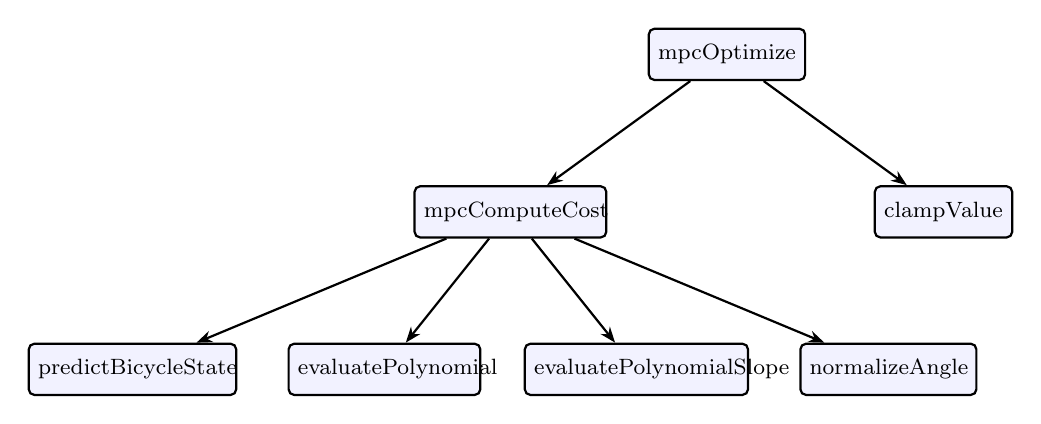
\begin{tikzpicture}[
  level 1/.style={sibling distance=5.5cm, level distance=2.0cm},
  level 2/.style={sibling distance=3.2cm, level distance=2.0cm},
  every node/.style={rectangle, draw, rounded corners=2pt, thick,
    minimum height=0.65cm, text centered, font=\footnotesize,
    fill=blue!5},
  edge from parent/.style={draw, -{Stealth[length=2mm]}, thick}
]

\node {mpcOptimize}
  child { node[text width=2.2cm] {mpcComputeCost}
    child { node[text width=2.4cm] {predictBicycleState} }
    child { node[text width=2.2cm] {evaluatePolynomial} }
    child { node[text width=2.6cm] {evaluatePolynomialSlope} }
    child { node[text width=2.0cm] {normalizeAngle} }
  }
  child { node {clampValue} };

\end{tikzpicture}
\end{center}

% ============================================================
%  1.7.x 下级函数需求
% ============================================================
\subsubsection{mpcComputeCost~---~MPC代价函数计算}

\begin{itemize}
  \item \textbf{功能}：计算给定控制序列下多步预测的 MPC 总代价，包含轨迹跟踪误差、控制幅值和控制变化率三部分。
  \item \textbf{输入}：控制序列、初始状态、参考轨迹、上周期控制量、MPC 参数。
  \item \textbf{输出}：double（总代价值）。
  \item \textbf{调用频次}：每次优化迭代调用 $4 N_c + 1$ 次（梯度计算 + 候选评估）。
\end{itemize}

\subsubsection{clampValue~---~数值限幅截断}

\begin{itemize}
  \item \textbf{功能}：将数值截断到闭区间 $[\text{minVal}, \text{maxVal}]$。
  \item \textbf{输入}：\texttt{value}, \texttt{minVal}, \texttt{maxVal}（double）。
  \item \textbf{输出}：double（截断后的值）。
  \item \textbf{用途}：施加转向角幅值约束、加速度幅值约束和转向角变化率约束。
\end{itemize}

% ============================================================
%  1.8 数据结构定义
% ============================================================
\subsection{数据结构定义}

以下数据结构定义于 \texttt{waypointFollowTypes.hpp} 和 \texttt{mpcOptimize.hpp}，命名空间 \texttt{waypoint\_follow}。

\subsubsection{VehicleState~---~车辆运动状态}
\begin{longtable}{|L{3.5cm}|C{2cm}|L{9.5cm}|}
\hline
\textbf{成员} & \textbf{类型} & \textbf{说明} \\
\hline
\texttt{x} & double & 纵向位置 (m) \\
\hline
\texttt{y} & double & 横向位置 (m) \\
\hline
\texttt{yaw} & double & 航向角 (rad)，逆时针为正 \\
\hline
\texttt{v} & double & 纵向速度 (m/s) \\
\hline
\end{longtable}

\subsubsection{ControlInput~---~车辆控制输入量}
\begin{longtable}{|L{3.5cm}|C{2cm}|L{9.5cm}|}
\hline
\textbf{成员} & \textbf{类型} & \textbf{说明} \\
\hline
\texttt{steeringAngle} & double & 前轮转向角 (rad)，左转为正 \\
\hline
\texttt{acceleration} & double & 纵向加速度 (m/s\textsuperscript{2})，加速为正 \\
\hline
\end{longtable}

\subsubsection{FittedTrajectory~---~拟合参考轨迹}
\begin{longtable}{|L{3.5cm}|C{2cm}|L{9.5cm}|}
\hline
\textbf{成员} & \textbf{类型} & \textbf{说明} \\
\hline
\texttt{poly} & PolynomialCoeffs & 归一化坐标系下的多项式系数 \\
\hline
\texttt{xOffset} & double & X坐标归一化偏移量 (m) \\
\hline
\texttt{xScale} & double & X坐标归一化缩放因子 (m) \\
\hline
\texttt{refSpeed} & double & 路点推算的参考车速 (m/s) \\
\hline
\texttt{valid} & bool & 轨迹拟合是否有效 \\
\hline
\end{longtable}

\subsubsection{MpcParam~---~MPC控制参数集}
\begin{longtable}{|L{4cm}|C{1.5cm}|C{1.5cm}|L{8cm}|}
\hline
\textbf{成员} & \textbf{类型} & \textbf{默认值} & \textbf{说明} \\
\hline
\endfirsthead
\hline
\textbf{成员} & \textbf{类型} & \textbf{默认值} & \textbf{说明} \\
\hline
\endhead
\texttt{predictionHorizon} & int & 15 & 预测步数 $N_p$ \\
\hline
\texttt{controlHorizon} & int & 5 & 控制步数 $N_c$ \\
\hline
\texttt{dt} & double & 0.1 & 预测时间步长 (s) \\
\hline
\texttt{wheelbase} & double & 2.85 & 前后轴距 (m) \\
\hline
\texttt{maxSteeringAngle} & double & 0.5236 & 前轮最大转向角 $\delta_{\max}$ (rad) \\
\hline
\texttt{maxAcceleration} & double & 3.0 & 最大纵向加速度 $a_{\max}$ (m/s\textsuperscript{2}) \\
\hline
\texttt{minAcceleration} & double & --5.0 & 最大纵向减速度 $a_{\min}$ (m/s\textsuperscript{2}) \\
\hline
\texttt{maxSteeringRate} & double & 0.05 & 每步最大转向角变化量 $\Delta\delta_{\max}$ (rad/step) \\
\hline
\texttt{maxOptIterations} & int & 30 & 梯度下降最大迭代次数 \\
\hline
\texttt{learningRate} & double & 0.5 & 梯度下降初始学习率 $\alpha_0$ \\
\hline
\texttt{finiteDiffEps} & double & $10^{-3}$ & 中心差分步长 $\varepsilon$ \\
\hline
\end{longtable}

\subsubsection{MpcOptimizeOutput~---~优化器输出}
\begin{longtable}{|L{4.5cm}|C{2.8cm}|L{7.7cm}|}
\hline
\textbf{成员} & \textbf{类型} & \textbf{说明} \\
\hline
\texttt{optimalSequence[15]} & ControlInput[15] & 优化后的控制序列 \\
\hline
\texttt{finalCost} & double & 优化后的代价值 \\
\hline
\end{longtable}

% ============================================================
%  1.9 测试用例
% ============================================================
\subsection{测试用例}

\subsubsection{正常测试用例}

{\small
\begin{longtable}{|C{0.6cm}|L{2.2cm}|L{4.8cm}|L{4.0cm}|L{3.5cm}|}
\hline
\textbf{编号} & \textbf{场景} & \textbf{输入} & \textbf{预期输出} & \textbf{验证准则} \\
\hline
\endfirsthead
\hline
\textbf{编号} & \textbf{场景} & \textbf{输入} & \textbf{预期输出} & \textbf{验证准则} \\
\hline
\endhead
N-1 &
直线轨迹优化 &
$v_0{=}20$, 直线轨迹, 暖启动全零 &
$\delta_k^* \approx 0$, $a_k^* \approx 0$, $J^*$ 接近零 &
$J^* \leq J^{(0)}$ \\
\hline
N-2 &
弯道轨迹优化 &
$v_0{=}15$, 圆弧轨迹 $R{=}100$\,m &
$\delta_k^* > 0$ (左转), $J^*$ 收敛 &
$J^* < J^{(0)}$ \\
\hline
N-3 &
暖启动效果 &
暖启动为上周期最优序列 &
收敛更快, $J^*$ 不高于冷启动 &
迭代次数 $\leq$ 冷启动 \\
\hline
N-4 &
约束饱和 &
极端弯道, 暖启动超约束 &
$|\delta_k^*| \leq \delta_{\max}$, $|\Delta\delta_k| \leq \Delta\delta_{\max}$ &
输出满足所有约束 \\
\hline
N-5 &
学习率衰减 &
困难场景, 代价多次上升 &
$\alpha$ 逐步衰减, $J^*$ 最终收敛 &
$J^*$ 有限, $\alpha < \alpha_0$ \\
\hline
\end{longtable}
}

\vspace{6pt}
{\small
\begin{longtable}{|L{2.5cm}|L{13cm}|}
\hline
\multicolumn{2}{|c|}{\textbf{正常测试用例符号说明}} \\
\hline
\textbf{符号} & \textbf{含义} \\
\hline
$v_0$ & 初始车速 initialState.v (m/s) \\
\hline
$\delta_k^*$ & 优化后转向角 optimalSequence[$k$].steeringAngle (rad) \\
\hline
$a_k^*$ & 优化后加速度 optimalSequence[$k$].acceleration (m/s\textsuperscript{2}) \\
\hline
$J^*$ & 最终代价值 finalCost \\
\hline
$J^{(0)}$ & 初始代价值（暖启动序列的代价） \\
\hline
$\delta_{\max}$ & 前轮最大转向角 maxSteeringAngle (rad) \\
\hline
$\Delta\delta_{\max}$ & 每步最大转向角变化量 maxSteeringRate (rad/step) \\
\hline
$\alpha$, $\alpha_0$ & 自适应学习率 / 初始学习率 \\
\hline
$R$ & 圆弧半径 (m) \\
\hline
\end{longtable}
}

\subsubsection{异常测试用例}

{\small
\begin{longtable}{|C{0.6cm}|L{2.0cm}|L{4.5cm}|L{4.2cm}|L{3.8cm}|}
\hline
\textbf{编号} & \textbf{场景} & \textbf{输入} & \textbf{预期输出/行为} & \textbf{验证准则} \\
\hline
\endfirsthead
\hline
\textbf{编号} & \textbf{场景} & \textbf{输入} & \textbf{预期输出/行为} & \textbf{验证准则} \\
\hline
\endhead
A-1 &
NaN 初始速度 &
$v_0{=}\text{NaN}$ &
不崩溃; 代价为 NaN, 序列保持暖启动 &
函数正常返回 \\
\hline
A-2 &
Infinity 初始速度 &
$v_0{=}+\infty$ &
代价发散; 学习率持续衰减 &
函数返回, 不崩溃 \\
\hline
A-3 &
零 xScale &
\texttt{trajectory.xScale}{$= 0$} &
代价计算除零; $J{=}\infty$ &
函数返回, 输出受约束 \\
\hline
A-4 &
无效轨迹 &
\texttt{trajectory.valid}{$=$}false, 系数全零 &
优化仍执行, 代价由速度项主导 &
函数正常返回 \\
\hline
A-5 &
零差分步长 &
$\varepsilon{=}0$ &
梯度计算除零: $0/0$ &
函数返回, 不崩溃 \\
\hline
A-6 &
极小差分步长 &
$\varepsilon{=}10^{-300}$ &
$J(u{+}\varepsilon) \approx J(u{-}\varepsilon)$, 梯度近零 &
优化几乎不更新 \\
\hline
A-7 &
零迭代次数 &
\texttt{maxOptIterations}{$= 0$} &
不迭代, 返回暖启动序列 &
$J^* = J^{(0)}$ \\
\hline
A-8 &
零控制步数 &
$N_c{=}0$ &
梯度循环不执行 &
返回空序列, $J^*{=}0$ \\
\hline
A-9 &
NaN 暖启动 &
warmStart[0].steeringAngle $=$ NaN &
NaN 传播到梯度计算 &
函数返回, 不崩溃 \\
\hline
A-10 &
极大暖启动值 &
warmStart 全 $\delta{=}100$\,rad &
约束投影裁剪到 $\delta_{\max}$ &
$|\delta_k^*| \leq \delta_{\max}$, $\forall k$ \\
\hline
\end{longtable}
}

\vspace{6pt}
{\small
\begin{longtable}{|L{2.5cm}|L{13cm}|}
\hline
\multicolumn{2}{|c|}{\textbf{异常测试用例符号说明}} \\
\hline
\textbf{符号} & \textbf{含义} \\
\hline
$v_0$ & 初始车速 initialState.v (m/s) \\
\hline
$\varepsilon$ & 中心差分步长 finiteDiffEps \\
\hline
$J^*$, $J^{(0)}$ & 最终代价值 / 初始代价值 \\
\hline
$N_c$ & 控制步数 controlHorizon \\
\hline
$\delta_k^*$ & 优化后转向角 (rad) \\
\hline
$\delta_{\max}$ & 前轮最大转向角 maxSteeringAngle (rad) \\
\hline
NaN & IEEE 754 非数值 (Not a Number) \\
\hline
$+\infty$ & IEEE 754 正无穷大 \\
\hline
\end{longtable}
}

\end{document}
